\documentclass{article}

\usepackage[english]{babel}
\usepackage{hyperref, float, amsmath}
\usepackage{tikz, xcolor, ifthen}
\usepackage{enumitem, caption, subcaption}

%\usepackage[list=off]{caption}

%\usepackage[inline, shortlabels]{enumitem}

\usetikzlibrary{fit, calc, arrows, shapes}

\newcommand{\red}[1]{{\color{red} #1}}
\newcommand{\green}[1]{{\color{green} #1}}
\newcommand{\yellow}[1]{{\color{yellow} #1}}



\begin{document}

% \begin{abstract}  % TODO
% \emph{University classes scheduling} is an old, well-known problem, that
% was attacked by the researches only recently, as the advances in electronics,
% made in the last 10--15 years, permitted construction of computational
% systems, far more advanced than \red{\dots}
% \end{abstract}

% Solutions to the problem are the \emph{university schedules}, that are
% composed of \emph{individual schedules} for each \emph{group} (\emph{student}),
% \emph{professor} and \emph{classroom}.

% Individual schedules are represented by \emph{timetables}, that hold one's
% \emph{classes} for a week. % TODO: rewrite this!
% A \emph{class} denotes some activity for a group of students under professor's
% supervision, that takes place in the classroom assigned. Actual activity and
% therefore the requirements, imposed on both professor and classroom, are defined by the
% \emph{discipline} in question.

\begin{abstract}

University classes scheduling problem consists in assigning
the \emph{classes}, defined by the academic program, for
each group of students, possibly taking in account participants' interests.

The problem is solved by agents negotiation over possible classes
configurations. The \emph{negotiating agents} are grouped by \emph{roles}:
\emph{professors} (\emph{full} and \emph{part time}), \emph{students} (\emph{groups}) and
\emph{classrooms}. Each agent has the knowledge, required by it's role.

The \emph{configuration} quality is assessed by it's \emph{coherence}.
A solution must exceed some quality threshold.

\end{abstract}

%\documentclass{article}


%\usepackage{xcolor, amsmath}
%\newcommand{\red}[1]{{\color{red} #1}}


\def\coh{\mathrm{coh}}


%\begin{document}

\section{Problem Formalization}

Let \begin{itemize}
\item $D=\{d_i\}$ be the set of \emph{disciplines}.
  A discipline may be seen as class descriptor, it contains
  academic program name and information about special requirements,
  such as laboratories.
\item $G=\{g_i\}$ be the set of \emph{groups}.
  A group unites some students. In this thesis it is assumed that
  \textbf{each student belongs strictly to one group}.
  A group has a set of disciplines, that it is obliged to take by an
  academical program.
\item $P=\{p_i\}$ be the set of \emph{professors}.
  Each professor can teach a set of disciplines, that is determined
  by the institution. There are two kinds of professors:
  \emph{full-time} and \emph{part-time}. The difference is that the
  latter have more flexible obligations, while the former have preference
  in classes assignment.
\item $R=\{r_i\}$ be the set of \emph{classrooms}.
  A classroom has two properties: capacity and special equipment installed.
\item $D=\{\bar d_i\}$ be the set of working \emph{days}.
\item $T=\{t_i\}$ be \emph{discrete time} (limited by working hours).
\end{itemize}
\medskip

A \emph{class} denotes an event \emph{discipline} for some \emph{group}
at some specific \emph{time interval} in the denoted \emph{classroom},
performed by some \emph{professor}.

$$ c \sim \left< d, g, p, r, \bar d, t, t \right> $$
\medskip

A \emph{candidate} to solution is a configuration (set) of classes.
It can be assessed by it's \emph{coherence}, that is properly discussed
in \ref{sectionCoherence}. Coherence is estimated within an agent and
depends on agent's knowledge.

\begin{align*}
 \tilde{c} &= \{c_i\}  &\coh[a]: \tilde c &\mapsto \Re
\end{align*}


The coherence function is designed in such a way, that given a candidate,
each agent, mentioned by candidate's underlying classes, yields the same
coherence assessment for the candidate.


\begin{align}
  \label{eq:coh-fun-independ}
  \begin{aligned}
    &\forall \tilde{c} = \{c_k\} \\
    &\forall c_i \sim \left< \dots, g_i, p_i, r_i, \dots \right> \\
    &\forall c_j \sim \left< \dots, g_j, p_j, r_j, \dots \right>
  \end{aligned}
& \implies
  \begin{aligned}
   \coh[g_i](\tilde c) &= \coh[g_j](\tilde c) = \\
   = \coh[p_i](\tilde c) &= \coh[p_j](\tilde c) = \\
   = \coh[r_i](\tilde c) &= \coh[r_j](\tilde c)
  \end{aligned}
\end{align}

\medskip

\noindent
The coherence function defines an order over the candidates and permits
agents to extract the \emph{acceptable} ones using a threshold.
The \textbf{negotiation goal} is to encounter an \emph{acceptable candidate}
for each negotiation participant.






%\end{document}

%\documentclass{article}


%\usepackage{hyperref, float, amsmath}
%\usepackage{tikz, ifthen, xcolor}
%\usepackage[english]{babel}

%\usetikzlibrary{fit, calc, arrows, shapes}

%\newcommand{\red}[1]{{\color{red} #1}}


%\begin{document}

\def\coh{\mathrm{coh}}
\def\cohi{\mathrm{\widetilde{coh}}}


\section{Coherence and Contexts}
\label{section:coherence}


Within an agent, the coherence is established over \emph{information graphs},
containing the assessed candidate's classes and \emph{context-specific
  knowledge} --- an \emph{information graph}, that holds the information,
already known/accepted by the agent.

The coherence concept and the idea of coherence-based agents
where taken from \cite{UAB-Thesis}, but the contexts and
coherence assessment were modified.

In \cite{UAB-Thesis} the best partition $\mathcal{A}$ \red{(called \emph{candidate} in this thesis)}
is obtained by an information graph $\mathcal{V}$, considering both
$\mathcal{A}$ and $\mathcal{V} \backslash \mathcal{A}$, as shown in figure
\ref{fig:UAB-partition}. The graph $\mathcal{V}$ is obtained by joining
contexts' graphs \cite[62]{UAB-Thesis}.

\begin{figure}[h]
  \label{fig:UAB-partition}
  \centering
  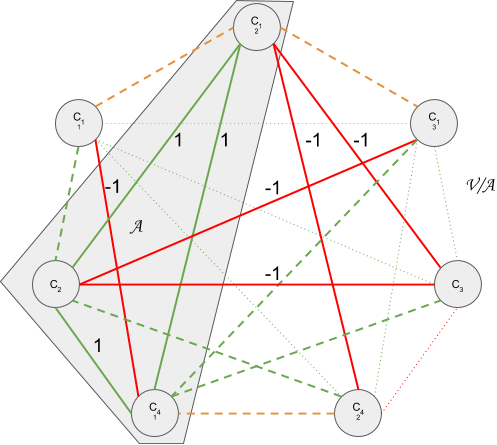
\includegraphics[width=0.5\textwidth]{img/UAB-splitting.png} % scale=0.5
  \captionsetup{singlelinecheck=off}
  \caption[caption]{ The coherence of partition $\mathcal{A},\mathcal{V}\backslash\mathcal{A}$
            is calculated in \cite{UAB-Thesis} as $
            \dfrac{ \text{\green{\emph{consistent}} relations in } \mathcal{A}
                  + \text{\red{\emph{inconsistent}} relations between }
                          \mathcal{A} \text{ and } \mathcal{V}\backslash\mathcal{A}}
                  {\text{total relations in } \mathcal{V}}$.
            \medskip\\ %\hspace{\textwidth}
            On the image above, the information graph $\mathcal{V}$ consists of
            classes $C_1,\dots,C_4$, also there are three possibilities for
            class $C_1$ placement and two for class $C_4$.

            A relation is
            \begin{itemize}[leftmargin=3cm]
              \item[\red{\emph{inconsistent}}], if two classes intersect in time;
              \item[\yellow{\emph{same class}}], if two classes differ only by time;
              \item[\green{\emph{consistent}}], otherwise.
            \end{itemize}

            Coherence of the partition is $\frac{|1| \cdot 3 + |-1| \cdot 5}
                                                {17} \approx 0.47$.
          }
\end{figure}


In this thesis, a different aproach is taken. The initial information graph,
composed of \emph{classes propositions}, is passed to a \emph{splitting} context,
that generates all posiible \emph{acceptable} (by the splitting context) sub-graphs,
called \emph{candidates} (as it will be shown in \emph{Beliefs} context).

Each candidate is propagated through the contexts in the established
order. At each context it gets assessed and the result is compared
against \emph{context-specific threshold}. If passing threshold test,
the candidate is sent to the next context, otherwise it is marked as failed
(providing a reason) and is propagated no further. In both cases the coherence
value is guarded alongside the candidate.

Thus a context in this thsis serves as \emph{candidates} filter.
\medskip

\noindent
A \emph{context} represents an aspect for optimization/restriction, considered
by an agent. It defines context-specific information and relations over the
information graph, with the corresponding combination functions. There are
two types of relations: \emph{binary} and over the \emph{whole graph}. The former ones
are applied to every pair of nodes and the results are combined by
\emph{binary fold functions} (one combines the results of the same relation
and the other combines the latter results). The whole-graph relations' values are
combined by the corresponding \emph{whole-graph fold function}. In the end the
combined values of both relations types are merged into the result by
\emph{combined merge function}. All the combination functions are defined at
contexts.

\begin{figure}[h]
  \centering
  \fbox{ 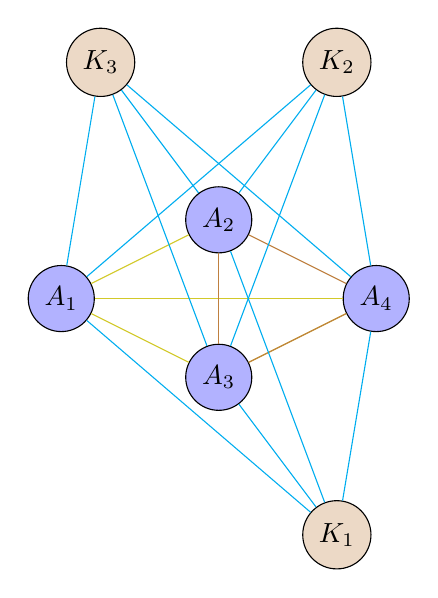
\begin{tikzpicture}

\tikzstyle{assessed}=[draw, circle, fill=blue!30];
\tikzstyle{innerKn}=[draw, circle, fill=brown!30];

\node[assessed] (a1) at (-2,0) {$A_1$};
\node[assessed] (a2) at (0, 1) {$A_2$};
\node[assessed] (a3) at (0,-1) {$A_3$};
\node[assessed] (a4) at (2, 0) {$A_4$};

\node[innerKn] (k1) at (1.5,-3) {$K_1$};
\node[innerKn] (k2) at (1.5, 3) {$K_2$};
\node[innerKn] (k3) at (-1.5,3) {$K_3$};

\begin{scope}[color=yellow!80!black]
 \foreach \i in {1,...,4}
  \foreach \j in {\i,...,4}{
   \ifthenelse{\NOT \(2 = \i \AND \(4 = \j \OR 3 = \j\)\) }
              { \draw (a\i) -- (a\j); }
              {}}
\end{scope}

\begin{scope}[color=brown]
 \foreach \i in {2,3,4}
  \foreach \j in {\i,...,4}
   \draw (a\i) -- (a\j);
\end{scope}

\begin{scope}[color=cyan]
 \foreach \i in {1,...,3}
  \foreach \j in {1,...,4}
   \draw (k\i) -- (a\j);
\end{scope}

\end{tikzpicture}

 }
  \caption{Binary relations within an information graph. One can
           distinguish the relations between the assessed information pieces
           and the relations between assessed and the known ones.
          }
\end{figure}


\subsection{Internal Contexts}

An internal context requires no knowledge from other agents.
The combined coherence of all the internal contexts is called
\emph{inner coherence} and is denoted as $\cohi$.

% % % % % % % % % % % % % % % % % % % % % % % % % % % % % % % % % % % % % % % %
\subsubsection{Capabilities}

Represent \emph{strong} restrictions, imposed by the institution.
All the relations should yield
\begin{itemize}
  \item [1], if the restriction is satistied;
  \item [0], otherwise.
\end{itemize}

Institution restrictions:
\begin{itemize}
\item \textbf{Group:} the candidate has the correct amount of classes for each
  discipline inscribed.
\item \textbf{Professor:} can teach every discipline assigned.
\item \textbf{Classroom:} has enough capacity and meets all special requirements.
\end{itemize}

An agent should be keeping the capabilities of known agents, to avoid creation
of unacceptable classes.

\begin{figure}[h]
  \centering
  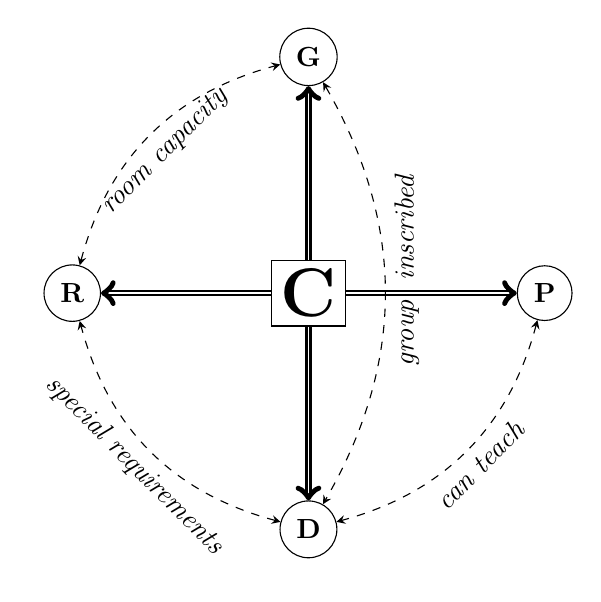
\begin{tikzpicture}
 
\edef\r{3cm}

\node[draw]         (C) at (0,  0) {\textbf{\Huge C}};
\node[draw, circle] (G) at (0, \r) {\textbf{G}};
\node[draw, circle] (P) at (\r, 0) {\textbf{P}};
\node[draw, circle] (D) at (0,-\r) {\textbf{D}};
\node[draw, circle] (R) at (-\r,0) {\textbf{R}};

\foreach \i in {(G),(P),(D),(R)}
 \draw[->, thick, double] (C) -- \i;

\def\data{ P/D/can teach
         , D/R/special requirements
         , R/G/room capacity
         , G/D/\quad~ group~~inscribed
         }

\foreach \i/\j/\k in \data
 \draw[<->, >=stealth, dashed] (\i) to[bend left
                                      ,edge node={node [sloped, below] {\emph{\k}}}]
                               (\j);


\end{tikzpicture}
  \caption{Capabilities required to form a \emph{class}.}
  \label{fig:capabilities}
\end{figure}


% % % % % % % % % % % % % % % % % % % % % % % % % % % % % % % % % % % % % % % %
\subsubsection{Beliefs (Time Consistency)}

Asserts that all the classes (concerning the assessing agent), are consistent in
time (do not intersect). This context is a splitting one, it uses the time
consistence relation to generate all possible time-consistent candidates from
given classes. It's internal knowledge should hold \emph{classes pool}, that
would be used for candidates generation via \emph{graph splitting}.
\\

The \emph{time consistence} relation yields following values:
\begin{itemize}[leftmargin=2cm]
  \item[-1], if two classes intersect in time (are inconsistent);
  \item[0], if two classes differ only by time
            (while have same discipline, group, professor and classroom);
  \item[1], otherwise (are consistent).
\end{itemize}


The splitting process uses context's relation \emph{aggregation} strategy.

\begin{align*}
  \mbox{Let } & C=\lbrace c \rbrace \text{ be the \emph{classes pool}}.\\
            ~ & A_i=\lbrace a_i \rbrace \text{ be a set of \emph{acceptable candidates},
                                         composed of } i \text{ classes.}\\
            ~ & A=\bigcup\limits_{i} A_i \text{ be a set of \emph{acceptable candidates}}.
\end{align*}

\begin{enumerate}
  \item Each single-class candidate is acceptable:
    $A_1 = \lbrace [ c ] ~||~ \forall ~ c \in C \rbrace$.
  \item Form $A_2$ by extending each candidate $[c'] = a_1 \in A_1$ with $c \in C$,
    if and only if $c'$ and $c$ are \emph{consistent in time}.
    If $A_1 \not= \emptyset$, then try to form $A_2$.
  \item[\vdots]
  \item[i.] Form $A_i$ by extending each candidate $[c'_1, \dots, c'_{i-1}] = a_{i-1}
    \in A_{i-1}$ with $c \in C$, if and only if $\forall c' \in a_{i-1}, ~c'$
    and $c$ are \emph{consistent in time}.
    If $A_i \not= \emptyset$, then try to form $A_{i+1}$.
   \item[\vdots]
   \item[n.] $A_n = \emptyset \implies$ all the \emph{acceptable candidates}
     were generated. Done.
\end{enumerate}


\begin{figure}[h]
  \label{fig:splittingCtx}
  \def\sfwidth{0.24\textwidth}
  \begin{subfigure}[b]{\sfwidth}
    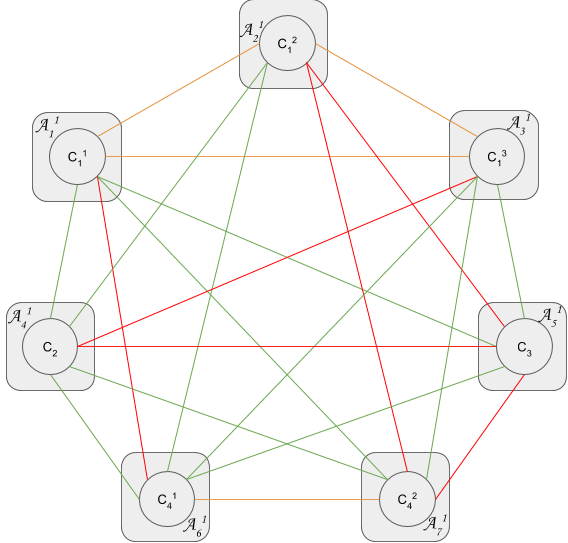
\includegraphics[width=\textwidth]{img/split-1-class.png}
    \caption{All single-class candidates are acceptable.}
  \end{subfigure}
  \begin{subfigure}[b]{\sfwidth}
    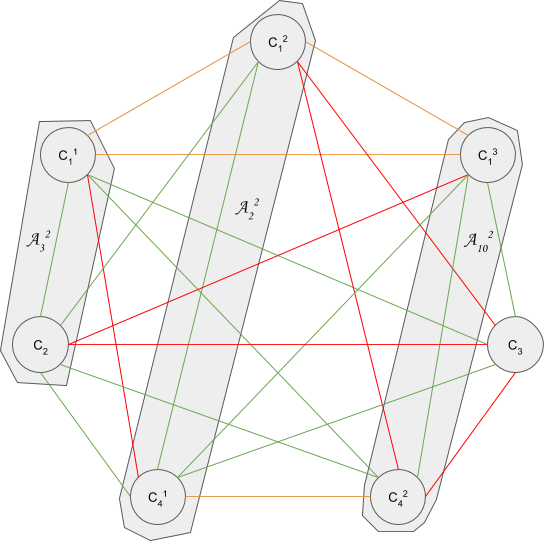
\includegraphics[width=\textwidth]{img/split-2-class_1.png}
    \caption[caption]{$\begin{aligned}
              A_3^2    &= A_1^1 + A_4^1\\
              A_2^2    &= A_2^1 + A_6^1\\
              A_{10}^2 &= A_3^1 + A_7^1
            \end{aligned}$}
  \end{subfigure}
  \begin{subfigure}[b]{\sfwidth}
    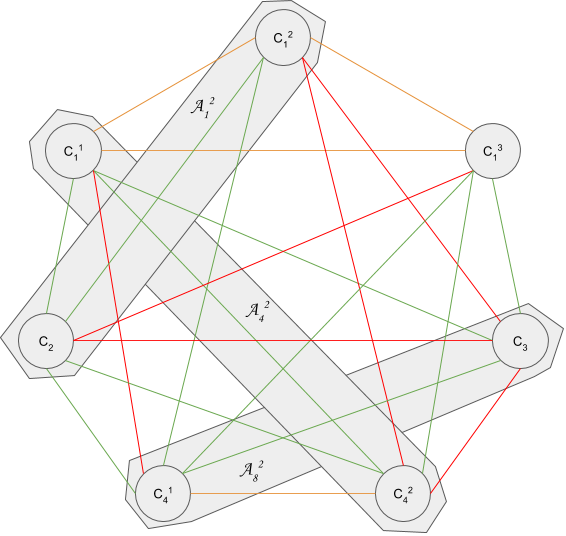
\includegraphics[width=\textwidth]{img/split-2-class_2.png}
    \caption[caption]{$\begin{aligned}
              A_1^2 &= A_2^1 + A_4^1\\
              A_4^2 &= A_1^1 + A_7^1\\
              A_8^2 &= A_5^1 + A_6^1
             \end{aligned}$}
  \end{subfigure}
  \begin{subfigure}[b]{\sfwidth}
    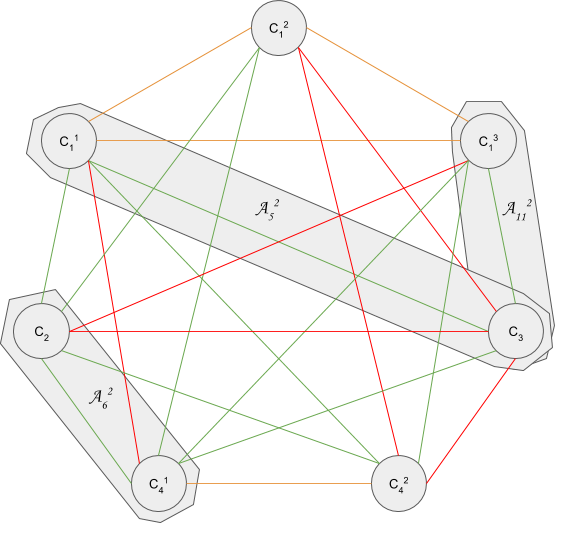
\includegraphics[width=\textwidth]{img/split-2-class_3.png}
    \caption[caption]{$\begin{aligned}
              A_5^2    &= A_1^1 + A_5^1\\
              A_{11}^2 &= A_3^1 + A_5^1\\
              A_6^2    &= A_4^1 + A_6^1
             \end{aligned}$}
  \end{subfigure}
\\
  \begin{subfigure}[b]{\sfwidth}
    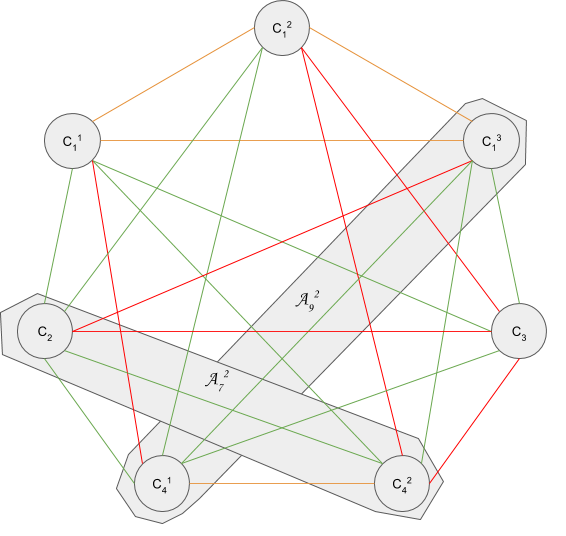
\includegraphics[width=\textwidth]{img/split-2-class_4.png}
    \caption[caption]{$\begin{aligned}
              A_7^2 &= A_4^1 + A_7^1\\
              A_9^2 &= A_3^1 + A_6^1
             \end{aligned}$}
  \end{subfigure}
  \begin{subfigure}[b]{\sfwidth}
    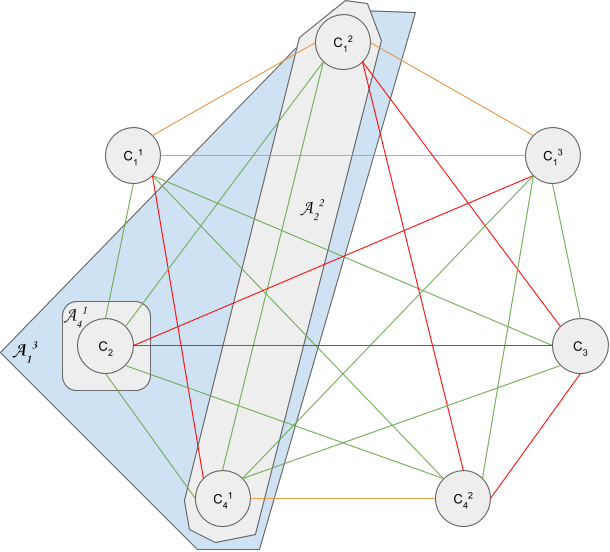
\includegraphics[width=\textwidth]{img/split-3-class_1.png}
    \caption[caption]{$\begin{aligned}
              A_1^3 &= A_2^2 + A_4^1\\
                    &= A_1^2 + A_6^1\\
                    &= A_6^2 + A_2^1
              \end{aligned}$}
  \end{subfigure}
  \begin{subfigure}[b]{\sfwidth}
    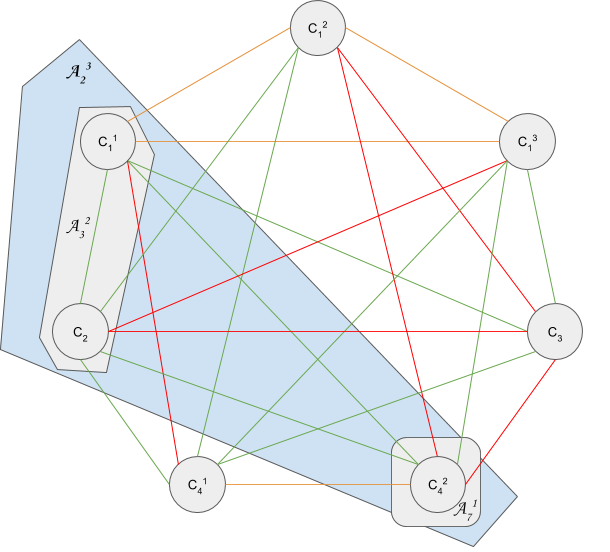
\includegraphics[width=\textwidth]{img/split-3-class_2.png}
    \caption[caption]{$\begin{aligned}
              A_2^3 &= A_3^2 + A_7^1\\
                    &= A_4^2 + A_4^1\\
                    &= A_7^2 + A_1^1
              \end{aligned}$}
  \end{subfigure}
  \begin{subfigure}[b]{\sfwidth}
    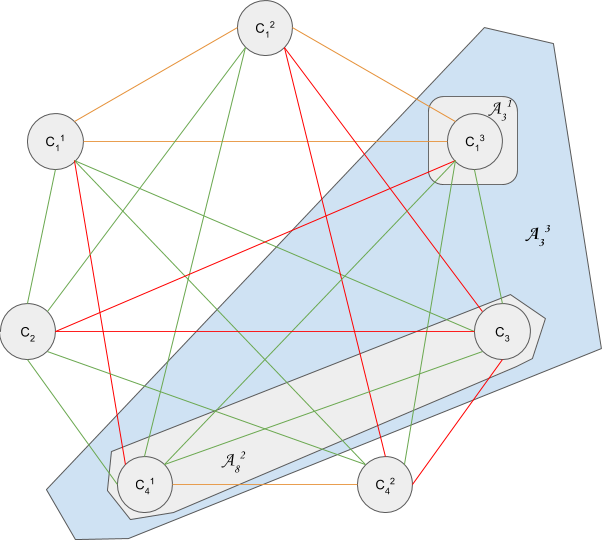
\includegraphics[width=\textwidth]{img/split-3-class_3.png}
    \caption[caption]{$\begin{aligned}
              A_3^3 &= A_8^2    + A_3^1\\
                    &= A_{11}^2 + A_6^1\\
                    &= A_9^2    + A_5^1
              \end{aligned}$}
  \end{subfigure}

  \caption{Information graph \emph{splitting} example. The graph is the same
           as in figure \ref{fig:UAB-partition}.
           There are in total \textbf{7}  1-class candidates,
                                    \textbf{11} 2-class candidates and
                                    \textbf{3}  3-class candidates.}
\end{figure}



% % % % % % % % % % % % % % % % % % % % % % % % % % % % % % % % % % % % % % % %
\subsubsection{Obligations}

The obligations determine custom \emph{strong restrictions} over the classes.
As in the case of \emph{capabilities}, the obligation relations must yield a
boolean result.

Possible \emph{obligation relations} examples: maximum classes per day,
lunch recess time, lower/upper class time limit, two classes must/cannot follow etc.

\red{At the moment there are no obligations used (but they are supported).}

% % % % % % % % % % % % % % % % % % % % % % % % % % % % % % % % % % % % % % % %
\subsubsection{Preference}

The preferences define \emph{weak restrictions}. The relations values might be any
value within $[0,1]$ interval. To avoid overrestrictions, this context's \emph{threshold}
should decrease with time.

\red{Possible preferences}

% % % % % % % % % % % % % % % % % % % % % % % % % % % % % % % % % % % % % % % %
\subsection{External}

The external context asks counterparts an \emph{opinion} about a candidate.
An opinion is the \emph{inner coherence} of the agent being asked.

\red{todo: images from g-drive ``ThesisCandidatesCommonGoal''}

%\end{document}

%\begin{document}


% \def\lifetime    {\mathit{lifetime}}
% \def\class       {\mathit{class}}
% \def\execute     {\mathit{execute}}
% \def\decide      {\mathit{decide}}
% \def\knownClasses{\overset{\mathrm{known}}{\mathit{classes}}}


\section{Agents and Negotiation}

The \emph{negotiating agents} are isolated proactive computational entities,
capable of sending and receiving messages.

The \emph{isolation} denotes that agents' internal states are protected
from outside access. Messaging is the only way an agent can be interacted with.
To ensure it, an agent is normally never interacted with directly, but
communicated via \emph{agent reference} instead.
The \emph{pro-activity} implies a capacity of acting asynchronously,
with no ``external'' cause.

Agents have \emph{roles}, that describe whom or what an agents represents
in the negotiation.

A negotiation has a \emph{classes pool}, distributed between the agents.
A class $\left< d, g, p, r, \bar d, t, t \right>$ is known to agents,
representing $g$, $p$ and $r$.

Negotiations are organized by special kind of agents --- \emph{controllers}.


\subsection{Agents}

In it's state an agent holds the \emph{run state} and special \emph{shared
  state}, called \emph{status}. The run state controls agent's execution
(and termination), while the status is monitored by the respective controller.
Agents have three \emph{run states}: ``Paused'', ``Running'' and ``Terminate''.
The first two states control pro-action; setting the last one causes all
agent's processes to stop. The \emph{status}es are further described in
section \ref{agentControllers}.

\subsubsection{Behavior}

Agent's behavior is flexible and may be changed during agent's lifetime.
It is determined by \emph{message handling} and \emph{action} functions.

An agent can simply \emph{send} a message, or it can \emph{ask} for some
\emph{expected response}, corresponding to the message sent. Agents have
separate handler functions for the two cases. All behavior functions
accept two arguments:
\begin{enumerate}
\item the agent's \emph{inner interface}, that provides
  control over agent's own behavior and lifetime;
\item agent's \emph{internal state}.
\end{enumerate}

Agents are executed in two computational threads: one for message handling
and another for proactive action.

\subsubsection{Coherence-based}

A \emph{coherence-based agent} bases its decisions on existing \emph{candidates}
and their \emph{coherence}. It must contain it's contexts within the state,
define contexts order and set the splitting one. It also must provide a
\emph{decider}.
\medskip

\noindent
Such agent acts repeatedly:
\begin{enumerate}
\item Gets its \emph{classes pool}, that may be stored within some context or
  somewhere else in the state.
\item Generates the initial candidates, using the \emph{splitting context} and
  classes pool.
\item Propagates the candidates through the contexts, as described in section
  \ref{section:coherence}.
\item Passes the \emph{assessed candidates} to the \emph{decider}.
\end{enumerate}

The decider must choose between two actions:
\begin{itemize}
\item Add new class(es) to the \emph{pool}. Such decision is taken if
  none of assessed candidates is \emph{acceptable}.
\item Select best solution and wait. This should be done if a satisfying
  solution was found. The agent's \emph{run state} is set to ``Paused'' and
  the \emph{status} is updated to ``Waiting''.
\end{itemize}

\subsubsection{Classes generation}
When no \emph{acceptable candidates} can be obtained by combining the classes
from the \emph{pool}, new class need to be added (to the \emph{classes pool}).

In order to avoid ``garbage'' classes generation, the newly created classes must:
\begin{itemize}
  \item Be \emph{capacity} consistent. The group, professor and classroom,
    assigned to the class, must be \emph{capable} of handling the assigned discipline
    (it must comply with their respective \emph{capabilities}).
  \item Not be a repetition of any of \emph{discarted classes}
    (see section \ref{section:clean-pool}).
\end{itemize}

\red{Furthermore, the generation \dots}

\subsubsection{Pool cleanup}
\label{section:clean-pool}
\red{TO DO}





\subsection{Controllers}

The controllers create new negotiating agents, and monitor their \emph{status}es
over their lifetimes. Controllers also provide communication references for the
agents they control. In order to facilitate references sharing, the controllers
are restricted to a single \emph{role} for it's agents.

Controllers have hierarchical structure, starting with the \emph{root
  controller}. The orders received by \emph{root} are propagated to
the underlying controllers.

\medskip

As mentioned before, negotiating agents have a special state,
called \emph{status}, that is monitored by the controllers. Apart
from receiving agents' errors, the \emph{status}es are used to
extract the \emph{distributed solution} from the agents.
This is done using ``Waiting'' and ``Locked'' statuses.

The agents set ``Waiting'' status when a suitable solution is found,
and the corresponding controller waits for all of its subjugated
agents to set it. When it is done, the controller sends ``Lock''
command to the agents and notifies the \emph{parent controller}.
When the \emph{root controller} receives ``Lock'' notifications from
all the controllers, it sends ``Collect'' order. On that order, the controllers
extract the solution parts (guarded in the statuses) and propagate them up to
the root.







% An agent is executing repetitively it's \emph{lifetime} function, while it remains
% capable of responding messages.

% \begin{align*}
%   \knownClasses &: \{\class_i\} \\
%   \lifetime &:~ \knownClasses \mapsto * \\
%   \lifetime &=  \execute \circ \decide \\
%   \decide   &:~ \knownClasses \mapsto
%               \mathrm{New\,candidate} ~|~
%               \mathrm{Ask\,acceptance} ~|~
%               \mathrm{Ask\,to\,yield}
% \end{align*}

% \subsection{New candidate}
% When no satisfying \emph{candidate} was found, new \emph{candidate}
% needs to be aggregated to the \emph{known classes}.
% The candidate must be \emph{internally coherent}.

% The newly created \emph{classes} (of which consists a candidate) are
% sent to the corresponding professor, group and classroom (except self).
% A confirmation, based on \emph{capabilities} must be received from all
% the candidates. Otherwise, another candidate must be generated.

% \textit{A cache might be used for the capabilities.}


% \subsection{Ask acceptance}
% When a candidate has no no contradiction at any context, an agent may decide to
% select it as it's part of solution and wait for the rest to do the same.
% It can be woken by a successful yield demand, forcing the waiting agent to
% search for a new solution.


% \subsection{Ask to yield}
% It is a solution when small percent of counterparts responded with a bad
% opinion (\emph{external} context) about a candidate. It asks them to yield
% to the candidate, that would mean (??) deleting (??) the contradicting classes
% in case of acceptance.  All asked agents must respond positively in order for
% the deletion to take place. In case of any refusal, the initial agent must
% (??) delete (??) the contradicting classes instead.

% The decision whether to yield or not is made considering the best inner
% coherence of any configuration, containing any contradicting class.

%\end{document}



\end{document}
